%
% LATEXBONES
%
\documentclass[a4paper,11pt,twoside]{article}
\usepackage{graphicx}
\usepackage{amsmath}
\usepackage[english]{babel}
\usepackage[applemac]{inputenc}
\usepackage[colorlinks,bookmarks=false,linkcolor=blue,urlcolor=blue]{hyperref}
\usepackage{subfigure}
\usepackage{here}
\usepackage{wrapfig}
\usepackage{fancyhdr}
\usepackage{dirtytalk}

%drow graph
\usepackage{fancybox}
\usepackage{tikz}
\usepackage{capt-of}

% print code
\usepackage{listings}
\usepackage{algorithm2e}
\usepackage{verbatim}

% push at the bottom
\newenvironment{bottompar}{\par\vspace*{\fill}}{\clearpage}

% landscape
\usepackage{pdflscape}

\paperheight=297mm
\paperwidth=210mm

\setlength{\textheight}{235mm}
\setlength{\topmargin}{-1.2cm} 

\setlength{\parindent}{0pt}

\setlength{\textwidth}{15cm}
\setlength{\oddsidemargin}{0.56cm}
\setlength{\evensidemargin}{0.56cm}

% quotes
\usepackage{framed}
\newcommand*{\signed}[1]{%
  \unskip\hspace*{1em plus 1fill}%
  \nolinebreak[3]\hspace*{\fill}\mbox{#1}
}

\pagestyle{plain}

% --- equations ---
\def \be {\begin{equation}}
\def \ee {\end{equation}}
%\def \dd  {{\rm d}}m

% --- links ---
\newcommand{\mail}[1]{{\href{mailto:#1}{#1}}}
\newcommand{\ftplink}[1]{{\href{ftp://#1}{#1}}}






% ======= Document ======

%----------------------------------------------------------------------------------------
% HEADING SECTIONS
%----------------------------------------------------------------------------------------

% --- header ---
\fancyhead[L]{Finance}
\fancyhead[R]{HW4}

\let\endtitlepage\relax

\begin{document}
\begin{titlepage} %Titre
\begin{center}
\newcommand{\HRule}{\rule{\linewidth}{0.5mm}} % Defines a new command for the horizontal lines, change thickness here
\center % Center everything on the page
 
 
 %----------------------------------------------------------------------------------------
% TITLE SECTION
%----------------------------------------------------------------------------------------




\begin{figure} [h] %----------- SubGraph ---------------------
\centerline{
\subfigure{
\includegraphics[height = 2 cm]{./pic/EPFL.png}  }
} 
\end{figure}

\HRule \\[0.4cm]
{ \huge \bfseries MGT-482 Principles of Finance \\Assignment 1}\\[0.4cm] % Title of your document

\begin{minipage}[t]{0.4\textwidth}
\flushleft
Prof. Erwan Morellec
\end{minipage}
~
\begin{minipage}[t]{0.55\textwidth}
\flushright
Team: \\
Joachim Muth - \mail{joachim.muth@epfl.ch}\\
Andreas Bill - \mail{andreas.bill@epfl.ch}\\
Nicolas Roth - \mail{nicolas.roth@epfl.ch}\\
\end{minipage}
\begin{center}
\today
\end{center}
\HRule \\
 %----------------------------------------------------------------------------------------

\end{center}
\end{titlepage}



\pagestyle{fancy}

% ================ Ex 1 ==============
\section{Part 1}

Table TAB\ref{table1} and figure FIG\ref{graph1} show that the equally-weighted portfolio has a very low volatility (between the lowest of the stocks) and a return equals to the mean of all the stocks it's composed by. Hence, with small risk, we can expect a goor return average.

\begin{center} %---------------Tab--------------
\begin{table}[H]
\centering
\begin{tabular}[h] {| l | l  l |}
\hline
& Mean annual return & Annual standard deviation\\
\hline
\hline
AAPL & 0.295204681  & 0.330266353 \\
C    & -0.061165009 & 0.519979071 \\
GE   & 0.074013637  & 0.289231592 \\
JNJ  & 0.099082103  & 0.140028396 \\
JPM  & 0.121412471  & 0.300971212 \\
MSFT & 0.122237352  & 0.249548908 \\
ORCL & 0.143860162  & 0.24154256  \\
PFE  & 0.083478109  & 0.189454886 \\
PG   & 0.069765875  & 0.153931446 \\
T    & 0.09555937   & 0.173152936 \\
WFC  & 0.134926001  & 0.319754747 \\
XOM  & 0.059770094  & 0.164580417 \\
\hline
Portfolio		&0.103178737			&0.177393884		\\
\hline
\end{tabular}
\label{table1}
\caption{Annual return and annual standard deviation for each stock and the equally-weighted portfolio}
\end{table}
\end{center}






\begin{figure}[H] %---------------------Graph---------------------------
\begin{center}
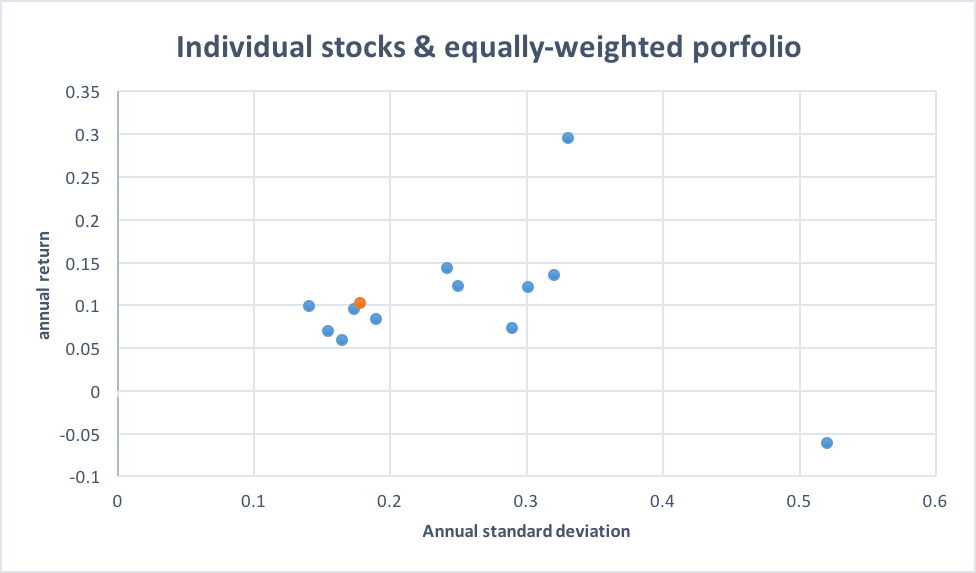
\includegraphics[width=12cm]{pic/graph_1.png} 
\end{center}
\caption{\em  \label{graph1}
Comparison between individual stocks return and variation and equally-weighted portfolio containing all of these stocks.
}
\end{figure}

																						


% ================ Ex 2 ==============
\section{Part 2}
Comparing tables TAB\ref{table_no_short} and TAB\ref{table_short} we notice that short sales allow use to decrease the volatility of a portfolio. The figure FIG\ref{graph2} illustrates this behavioure, indeed, we can see that for a same return the curve is shifted one the left, which means lower standard deviation of the return.

Let's notice that in table TAB\ref{table_no_short} there are no weights provided for a portfolio return of 40\% because the Excel Solver was not able to find a solution. Indeed, a look at table TAG\ref{table1} show us that the stock with more return is AAPL, with a return of 29.52\% then, even by having a portfolio containing 100\% of this stock we cannot acchieve the desired 40\% of return.

\begin{center} %---------------Tab--------------
\begin{table}[H]
\centering
\begin{tabular}{| l | llllllll |}
\hline
& 0.9  & 0.11   & 0.13   & 0.15   & 0.2    & 0.25   & 0.3    & 0.4 \\
\hline
\hline
AAPL & 0.0243 & 0.0990 & 0.1731 & 0.2532 & 0.4990 & 0.7472 & 1.0000 & - \\
C    & 0.0000 & 0.0000 & 0.0000 & 0.0000 & 0.0000 & 0.0000 & 0.0000 & - \\
GE   & 0.0000 & 0.0000 & 0.0000 & 0.0000 & 0.0000 & 0.0000 & 0.0000 & - \\
JNJ  & 0.3786 & 0.4426 & 0.5049 & 0.5419 & 0.4158 & 0.1309 & 0.0000 & - \\
JPM  & 0.0000 & 0.0000 & 0.0000 & 0.0000 & 0.0000 & 0.0000 & 0.0000 & - \\
MSFT & 0.0000 & 0.0000 & 0.0000 & 0.0000 & 0.0000 & 0.0000 & 0.0000 & - \\
ORCL & 0.0000 & 0.0002 & 0.0002 & 0.0002 & 0.0002 & 0.0000 & 0.0000 & - \\
PFE  & 0.0255 & 0.0182 & 0.0108 & 0.0000 & 0.0000 & 0.0000 & 0.0000 & - \\
PG   & 0.1645 & 0.1068 & 0.0458 & 0.0000 & 0.0000 & 0.0000 & 0.0000 & - \\
T    & 0.2064 & 0.1939 & 0.1816 & 0.1546 & 0.0000 & 0.0000 & 0.0000 & - \\
WFC  & 0.0000 & 0.0143 & 0.0318 & 0.0501 & 0.0850 & 0.1219 & 0.0000 & - \\
XOM  & 0.2008 & 0.1250 & 0.0518 & 0.0000 & 0.0000 & 0.0000 & 0.0000 & -\\ 
\hline
\end{tabular}\label{table_no_short}
\caption{Weight of each stock for optimal portfolio with \emph{no short sales} constraint}
\end{table}
\end{center}

\begin{center} %---------------Tab--------------
\begin{table}[H]
\centering
\begin{tabular}{| l | llllllll |}
\hline
& 0.9  & 0.11    & 0.13    & 0.15    & 0.2     & 0.25    & 0.3     & 0.4     \\
\hline
\hline
AAPL & -0.0345 & 0.0133  & 0.0603  & 0.1042  & 0.2198  & 0.3354  & 0.4499  & 0.6786  \\
C    & -0.0481 & -0.0834 & -0.1190 & -0.1546 & -0.2434 & -0.3320 & -0.4213 & -0.5994 \\
GE   & -0.1844 & -0.1906 & -0.1969 & -0.2031 & -0.2185 & -0.2342 & -0.2501 & -0.2830 \\
JNJ  & 0.3143  & 0.3555  & 0.3965  & 0.4307  & 0.5270  & 0.6247  & 0.7196  & 0.9100  \\
JPM  & 0.0333  & 0.0484  & 0.0659  & 0.0792  & 0.1174  & 0.1558  & 0.1926  & 0.2663  \\
MSFT & 0.0331  & 0.0294  & 0.0264  & 0.0203  & 0.0099  & -0.0015 & -0.0019 & -0.0019 \\
ORCL & 0.0029  & 0.0030  & 0.0038  & 0.0218  & 0.0375  & 0.0535  & 0.0668  & 0.0934  \\
PFE  & 0.0291  & 0.0288  & 0.0262  & 0.0264  & 0.0260  & 0.0218  & 0.0228  & 0.0214  \\
PG   & 0.2435  & 0.1945  & 0.1459  & 0.1013  & -0.0175 & -0.1355 & -0.2552 & -0.4943 \\
T    & 0.2435  & 0.2331  & 0.2229  & 0.2095  & 0.1807  & 0.1529  & 0.1216  & 0.0617  \\
WFC  & 0.0877  & 0.1293  & 0.1700  & 0.2107  & 0.3129  & 0.4158  & 0.5178  & 0.7225  \\
XOM  & 0.2796  & 0.2388  & 0.1981  & 0.1535  & 0.0483  & -0.0565 & -0.1626 & -0.3754 \\ 
\hline
\end{tabular}\label{table_short}
\caption{Weight of each stock for optimal portfolio with no constraint}
\end{table}
\end{center}




\begin{figure}[H] %---------------------Graph---------------------------
\begin{center}
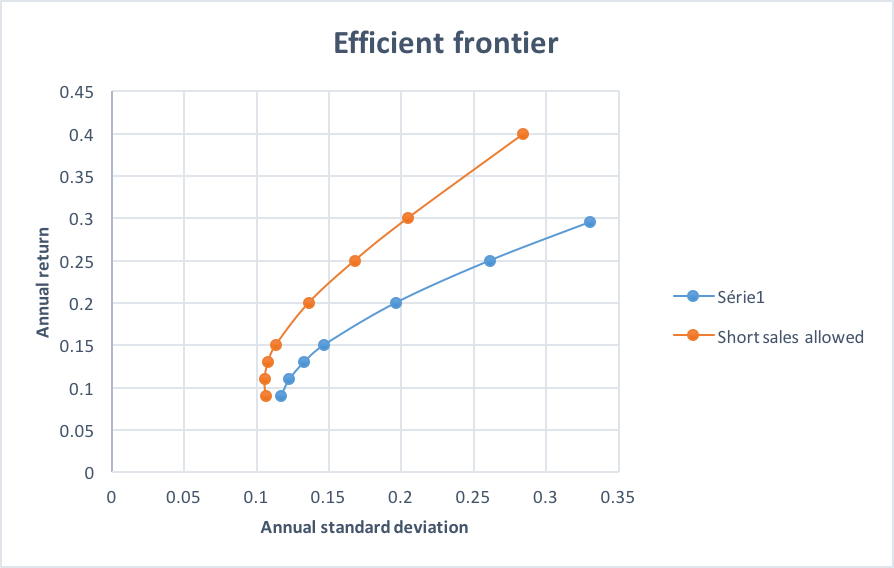
\includegraphics[width=12cm]{pic/graph_2.png} 
\end{center}
\caption{\em  \label{graph2}
Efficient frontiers for constrained and non-constrained portfolio.
}
\end{figure}



% ================ Ex 3 ==============
\section{Part 3}


\begin{center} %---------------Tab--------------
\begin{table}[H]
\centering
\begin{tabular}{| l | lllllll | }
\hline
& Constante & Slope   & Slope t-stat & adj. $R^2$ & n. obs. & Jensen's $\alpha$ & $E[R_i]$        \\
\hline
\hline
AAPL      & 0.0186  & 1.2145       & 7.2404             & 0.3035          & 119            & 0.0229          & 0.0672 \\
C         & -0.0167 & 2.3711       & 10.3059            & 0.4714          & 119            & 0.0107          & 0.1122 \\
GE        & -0.0012 & 1.5061       & 13.8316            & 0.6173          & 119            & 0.0089          & 0.0785 \\
JNJ       & -0.0012 & 1.5061       & 13.8316            & 0.6173          & 119            & 0.0089          & 0.0785 \\
JPM       & 0.0053  & 0.6034       & 9.2967             & 0.4199          & 119            & -0.0026         & 0.0434 \\
MSFT      & 0.0051  & 1.0336       & 8.6950             & 0.3873          & 119            & 0.0058          & 0.0602 \\
ORCL      & 0.0065  & 1.1132       & 10.5183            & 0.4816          & 119            & 0.0088          & 0.0633 \\
PFE       & 0.0032  & 0.7586       & 8.2347             & 0.3615          & 119            & -0.0016         & 0.0495 \\
PG        & 0.0032  & 0.5250       & 6.5148             & 0.2599          & 119            & -0.0063         & 0.0404 \\
T         & 0.0052  & 0.5727       & 6.2508             & 0.2439          & 119            & -0.0034         & 0.0423 \\
WFC       & 0.0053  & 1.2198       & 7.6430             & 0.3273          & 119            & 0.0097          & 0.0674 \\
XOM       & 0.0020  & 0.6034       & 7.2086             & 0.3016          & 119            & -0.0059         & 0.0434 \\
\hline
\end{tabular}
\label{table_short}
\caption{Correlation and statistical analysis of the stock with S\&P500.}
\end{table}
\end{center}


The $\beta$ slope coefficient represent the correlation between return of the S\&P 500 index and return of each of the stocks. I.e. for a grow in return of 10\% in S\&P 500 index and AAPL $\beta$\% $=1.2$, this means a growth of 12\% of the AAPL return.

Adj. $R^2$ is a statistical value that gives us the trust we can have in the $\beta$ coefficient. The higher $R^2$ is, the more correlation exists between S\&P 500 and the stock, the more we can expect both of them to have the same behaviour.

Jensen?s $\alpha$ measures the performance of the stock during the regression period. To compute it, we used the following formula :

$$Jensens \alpha = \alpha_i - rf \cdot (1 - \beta_i) $$

Its value can be interpreted as follows :
\begin{itemize}
\item $\alpha > 0$, then the stock did better than expected
\item $\alpha < 0$, then the stock did worse than expected
\item $\alpha = 0$, then the stock did exactly as expected
\end{itemize}

Looking at the expected return of the stocks and using the formula:
$$r_{premium} = return - r_f$$
a 4.5\% risk premium seems reasonable.



%======= TABLEAU ===========
%\begin{center} %---------------Tab--------------
%\begin{tabular} {| c | c | c | c | c | c |}
%\hline
 %& & & & & $\\ \hline
%\end{tabular}
%\end{center}


%===========GRAPH================
%\begin{figure} %---------------------Graph---------------------------
%\begin{center}
%\includegraphics[width=12cm]{graph/ampli2} 
%\end{center}
%\caption{\em  \label{label}
%L�gende
%}
%\end{figure}


%========SUBGRAPH=======
%\begin{figure} [h] %----------- SubGraph ---------------------
%\centerline{
%\subfigure[ sublegend ] {\label{sfig:thetat} \includegraphics[width=7cm]{ graph/graph_convdt3 } }
%\subfigure[ sublegend ] {\label{sfig:thetafin} \includegraphics[width=7cm]{ graph/graph_convtfin } } 
%}
%\caption{\label{ label } 
%L�gende
%} 
%\end{figure}








\end{document} %%%% THE END %%%%
